
\documentclass[a4paper,12pt]{article} % тип документа


% Русский язык
\usepackage[T2A]{fontenc} % кодировка
\usepackage[utf8]{inputenc} % кодировка исходного текста
\usepackage[russian,english]{babel} % локализация и переносы
\usepackage{graphicx}
\graphicspath{{pictures/}}
\DeclareGraphicsExtensions{.pdf,.png,.jpg}


% Математика
\usepackage{amsmath,amsfonts,amssymb,amsthm,mathtools}


\usepackage{wasysym}

%Заговолок
\author{Талашкевич Даниил Александрович}

\title{Лабораторная работа 1.2.1}

\date{\today}

\begin{document}

\maketitle
\thispagestyle{empty}

\newpage
\setcounter{page}{1}

\begin{center}
{\bf 1. Аннотация}
\end{center}

В данной работе мы определяем скорость полета пули, применяя законы сохранения и используя баллистические маятники.

\begin{center}
{\bf 2. Используемое оборудование}
\end{center}

Духовое ружье на штативе, осветитель, оптическая система для измерения отклонений маятника, измерительная линейка, пули и весы для их взвешивания, пинцет, а также баллистические маятники.

\begin{center}
{\bf 3. Теоретические сведения}
\end{center}

Скорость вылета пули из духового ружья $150-200 \ \frac{\textbf{м}}{\textbf{с}}$, из боевой винтовки $\sim 1000 \ \frac{\textbf{м}}{\textbf{с}}$.\\
Это скорости большие по сравнению, скажем, со скоростью пешехода $(\sim 2 \ \frac{\textbf{м}}{\textbf{с}})$ или даже $(\sim 20 \ \frac{\textbf{м}}{\textbf{с}})$. Поскольку размер лабораторной установки обычно порядка нескольких метров, время пролета пули составляет величину порядка $10^{-2} - 10^{-3} c.$ Для измерения таких величин необходима дорогостоящая аппаратура, регистрирующая быстропеременные процессы. Дешевле определить скорость пули по импульсу, передаваемому ею некоторому телу при неупругом соударении. В отсутсвие внешних сил, а при кратковременном ударе даже и при действии внешних сил, а при кратковременном ударе даже и при действии внешних сил, импульс системы пуля--тело сохраняется. Если масса тела значительно больше массы пули, то скорость тела с застрявшей в нем пулей будет значительно меньше скорости пули, и ее легче измерить. Длительность неупругого соударения пули и тела, измеряемая с моментах их соприкосновения до прекращения относительного движения, зависит от сопротивления, которое испытывает пуля при движении внутри тела. Оценить ее можно по глубине про-
никновения пули в тело. предполагая силу сопротивления постоянной.
Если при скорости $200$ м/c глубина проникновения $\sim$ 1 см, то время
соударения $\sim 10^{-4}$ с. За это время даже тело только в $100$ раз более
тяжелое, чем пуля, сдвинется всего на $0,1$ мм. При малых временах
соударения внешние силы конечной величины сообщают импульс, на-
много меныший импульса. пули.

Для измерения переданного пулей импульса и, следовательно, ее
скорости используют баллистический маятник. Баллистическим назы-
вается маятник, колебания которого вызываются кратковременным на-
чальным импульсом (толчком). Кратковременным можно считать им-
пульс, если время действия сил (время соударения) значительно мень-
ше периода колебаний маятника. При этом отклонение маятника за,
время соударения значительно меньше амплитуды колебаний — мак-
симального отклонения маятника. В случае гармонических колебаний
время соударения $\tau$, отнесенное к периоду колебаний $T$, и отклонение
$\Delta \varphi$ за время соударения, отнесенное к максимальному отклонению фт
(амплитуде), связаны простым соотношением \[ \frac{\Delta\varphi}{\varphi}_{m} \approx \frac{2\pi \tau}{T}.\]

В результате если время соударения составляет 0,01 периода, то откло-
нение равно 0,06 максимального отклонения.

Связь между максимальным отклонением маятника и начальной скоростью, полученной им в результате толчка, описывается законом сохранения механической энергии, если потери энергии за. период значительно меньше энергии его колебаний. В дальнейшем будем считать затухание малым, если за, десять колебаний амплитуда, уменьшается меньше, чем наполовину. По начальному максимальному отклонению
маятника определяются импульс и скорость пули.

При проведении эксперимента. необходимо позаботиться о том, чго-
бы после удара, пули колебания маятника происходили в одной плос-
кости и отсутствовали поперечные движения. Достигается это соответ-
ствующей установкой ружья. При этом надо иметь в виду. что вслед
за пулей из ружья выходит воздушная струя. которая может оказать
влияние на движение маятника, и исказить результаты опыта. Поэтому
ружье должно располагаться на. расстоянии. достаточном для растека-
ния струи. Влияние струи газов на. маятник можно оценить с помощью
холостого выстрела.

Ружье закреплено на специальном штативе. Чтобы зарядить ружье, надо освободить стопорный винт штатива и наклонить ружье в держатель набок. Затем отогнуть ствол в сторону курка до упора. зарядив ружье, все вернуть в первоначальное состояние.
\newpage
\begin{center}
{\bf 4. Экспериментальная установка}
\end{center}

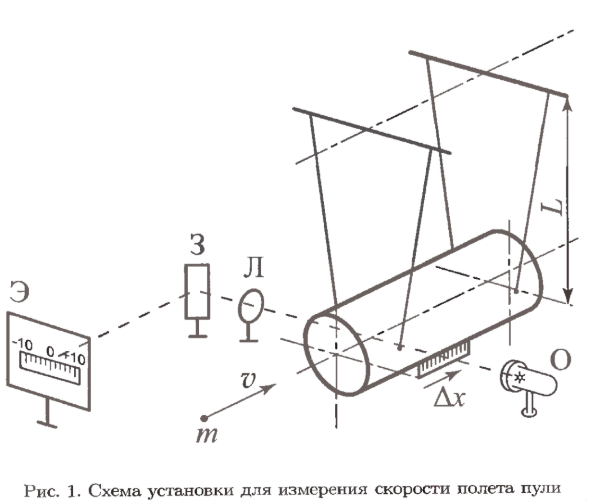
\includegraphics[width=\textwidth]{1.2.1 1}

\begin{center}
{\bf 5. Метод баллистического маятника, совершающего
поступательное движение.}
\end{center}

Используемый в этой части работы баллистический маятник пред-
ставляет собой тяжелый цилиндр, подвешенный на четырех нитях оди-
наковой длины. Он изображен на. рис. 1 вместе с измерительной си-
стемой. Любая точка цилиндра при колебаниях маятника, движется по
дуге окружности, радиус которой равен расстоянию по вертикали меж-
ду уровнями верхнего и нижнего концов нитей подвеса. Это поясняет-
ся на рис. 2 (вид сбоку, в плоскости колебаний). Все точки цилиндра
движутся по дугам окружностей одинакового радиуса относительно
соответствующих каждой точке центров, в частности, центр масс $M_0$
переходит в $M_1$ по дуге окружности с центром в точке $O$. Все радиусы
одинаковы и обозначены $L$.

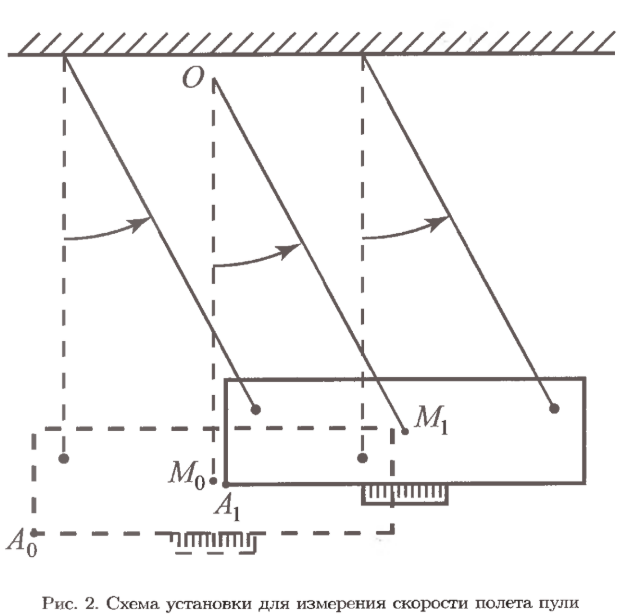
\includegraphics[width=\textwidth]{1.2.1 2}

Выше уже говорилось о требованиях к установке ружья. В данном
случае его необходимо установить таким образом, чтобы скорость пу-
ли перед ударом была направлена горизонтально вдоль оси цилиндра
(по крайней мере, достаточно близко к этому). Внешними силами для системы пуля-цилиндр являются сила тяжести, которая не имеет горизонтальной компоненты, и силы натяжения нитей, у которых появляются горизонтальные компоненты при отклонения малы, то и эти компоненты малы. Тем более мал по сравнению с импульсом пули их импульс за время соударения. Поэтому закон сохранения импульса при соударении пули с цилиндром имеет вид \[ mu = (M + m) V.\]

Здесь $m$ -- это масса пули, $M$ -- масса цилиндра, $u$ -- скорость пули перед ударом, $V$ --  скорость цилиндра и пули после неупругого соударения.

Учитывая, что масса маятника значительно больше массы пули, можно написать \[ u = \frac{M}{m}V.\]

Получив начальную кинетическую энергию, матяник при отклонении будет подниматься до тех пор, пока всю ее не израсходует. Если пренебречь потерями, то вся кинетическая энергия переходит в потенциальную в поле тяжести. Тогда по закону сохранения механической энергии высота $h$ подъема маятника над его начальным положением связана с начальной скоростью маятника $V$ следующим образом : \[ V^2 = 2gh.\]

Здесь $g$ -- ускорения свободного падения.

Высота подъема маятника выражается через угол $\varphi$ отклонения маятника от вертикали: \[ h = L(1 - \cos{\varphi}) = 2L \sin^2{\frac{\varphi}{2}}, \textbf{ где } \varphi \approx \frac{\Delta x}{L}.\]

Из всех вышеперечисленных получаем окончательную формулу для определения скорости пули:\[ u = \frac{M}{m}\sqrt{\frac{g}{L}}\Delta x.\]

Измерение отклонения маятника $\Delta x$ производится с помощью оптической системы, изображенной на рис. 1. По увеличенному изображению шкалы, закрепленной на цилиндре, определяется ее горизонтальное смещение. Таким образом может быть измерено максимальное отклонение маятника и изменение максимальных отклонений для определения затуханий колебаний.

Справедливость соотношения для $V^2 = 2gh$ и, следовательно, окончательной формулы обусловлена возможность пренебречь потерями энергии при колебаниях.

Среди причин, вызывающих затухание колебаний маятника, наиболее существенными являются трение о воздух и недостаточно жесткое закрепление точки подвеса.

Если потери энергии за четверть периода колебаний малы по сравнению с максимальной потенциальной энергией, которую маятник при этом приобретает, то их можно не учитывать в законе сохранения. Как уже говорилось, затуханием можно пренебречь, если за десять периодов амплитуда колебаний уменьшается меньше, чем в два раза.
\newpage

\begin{center}
{\bf Ход работы}
\end{center}

\begin{center}
{\bf 1. Ознакомление с оборудованием.}
\end{center}

Ознакомимся с устройством баллистического маятника и измерительной установки,так же научимся пользоваться духовным ружьем.

\begin{center}
{\bf 2. Измерение масс пуль}
\end{center}

Измерим на аналитических весах массу каждой пульки, полученной у лаборанта, поместим их в ячейки коробки под соответствующими номерами, чтобы не перепутать при использовании. Данные измерения привидены в таблице ниже:

\begin{center}
\begin{tabular}{|c|c|c|c|c|c|c|c|c|}
\hline 
m, гр & 0.511 & 0.507 & 0.496 & 0.500 & 0.509 & 0.510 & 0.500 & 0.505 \\ 
\hline 
N & 1 & 2 & 3 & 4 & 5 & 6 & 7 & 8\\ 
\hline 
\end{tabular} 
\end{center}

Первые четыре грузика будут учавствовать в первой части лабораторной работы, а другие четыре во второй соответственно.

\begin{center}
{\bf 3. Измерение данных установки}
\end{center}

С помощью 2-х метровой линейки измеряем расстояние $L$(см. рис.1) . Полученные значения:
\begin{center}
\begin{tabular}{|c|c|c|c|c|c|}
\hline 
L, см  & 220 & 220 & 220 & 220 & 220\\ 
\hline 
\end{tabular} 
\end{center}

C учетом погрешности линейки получим : $\langle L\rangle = 220 \pm 1 \textbf{см}$. 

Так же $M = 2925 \pm 5 $гр.

\begin{center}
{\bf 4. Сборка оптической системы}
\end{center}

Собираем оптическую систему, предназначенную для измерения перемещения маятника. Включаем осветитель и добиваемся четкого изображения шкалы на экране.

\begin{center}
{\bf 5. Проверка влияния холостых выстрелов и приверка милы ли колебния}
\end{center}

После произведения нескольких холостых выстрелов по маятнику я убедился, что влияние полностью отсутствует. Так же после 10 колебаний амплитуда уменьшилась в $\frac{12,7 - 12}{12,7} \approx 5\% \langle 50\% $ -- отсюда вывод, что затухание колебаний мало.
\newpage
\begin{center}
{\bf 6. Выстрели пуль}
\end{center}

Проводим выстрелы пуль из ружья, при этом замеряя отклонения $\Delta x$. Построим таблицу полученных данных:

\begin{center}
\begin{tabular}{|c|c|c|c|c|}
\hline 
$N$ & 1 & 2 & 3 & 4 \\ 
\hline 
$m$, гр & 0.511 & 0.507 & 0.496 & 0.5 \\ 
\hline 
$\Delta x$, мм & 12,9 & 12,8 & 12,5 & 12,6 \\ 
\hline 
\end{tabular} 
\end{center}

\begin{center}
{\bf 7. Оценка погрешности и среднего значения}
\end{center}

Рассчитаем значение скорости для разных выстрелов по формуле из теоретического введения $u = \frac{M}{m}\sqrt{\frac{g}{L}}\Delta x$:

\begin{center}
\begin{tabular}{|c|c|c|c|c|}
\hline 
$N$ & 1 & 2 & 3 & 4 \\ 
\hline 
$m$, гр & 0.511 & 0.507 & 0.496 & 0.5 \\ 
\hline 
$\Delta x$, мм & 12,9 & 12,8 & 12,5 & 12,6 \\ 
\hline 
$u$, м/с  & 157.4 & 157.4 & 157.2 & 157.2 \\ 
\hline
\end{tabular} 
\end{center}

Погрешность измерений $\Delta x = 0.05\cdot 10^{-3}$ м, погрешность измерений $\Delta m = 0.001$ гр, погрешность $\Delta M = 5$ гр, погрешность $\Delta L = 0.01$ м. Среднее значение $\langle u\rangle\ =\ 157.3$ м/с. Общая погрешность $u$ :

$\sigma_{\textbf{абс}} = \sqrt{\sigma_{\textbf{сл}} + \sigma_{u}}$.

$\sigma_{\textbf{сл}} = \sqrt{\frac{\sum\limits_{i = 1}^{N}(\Delta X_i)^2}{N\cdot (N - 1)}}$, где $\Delta X_i = (X_{cp} - X_i)$. 

\[\sigma_u = \sqrt{(\frac{\sigma u}{\sigma a})^2\cdot \sigma_a^2 + (\frac{\sigma u}{\sigma b})^2\cdot \sigma_b^2 + \cdots}.\]

Оценка погрешности определения скорости пули в каждом выстреле:

\[ \sigma_u = \sqrt{\frac{g\Delta x^2}{m^2L}\cdot \sigma_M^2 + \frac{M^2g\Delta x^2}{4m^2L^3}\cdot \sigma_L^2 + \frac{M^2g}{m^2L}\cdot \sigma_x^2 + \frac{M^2\Delta x^2g}{L^2 m^4}\cdot \sigma_m^2}.\]

Так как $\Delta x^2 \rightarrow 0$, то всеми слагаемыми с $\Delta x^2$ можно пренебречь. Получаем : \[ \sigma_u = \sqrt{\frac{M^2g}{m^2L}\cdot \sigma_x^2} .\]

По полученным данным имеем:

\[ \sigma_u =  \sqrt{\frac{2.925^2 \cdot 10}{0.504^2\cdot 10^{-6} \cdot 2.2}\cdot 0.05^2\cdot 10^{-6}} = 0.61 \textbf{ м/с}.\]

\[ \sigma_{\textbf{сл}} = 0.06\textbf{ м/с}.\] 

\[ \sigma_{\textbf{абс}} = \sqrt{0.06^2 + 0.61^2} = 0.62 .\]

Отсюда $u = 157.3 \pm 0.62 \textbf{ м/с}$.

\begin{center}
{\bf 8. Вывод о наблюдаемом разбросе и объяснение с чем это связано? ошибка опыта или различием скоростей от выстрела к выстрелу.}
\end{center}

Оценка разброса отдельных результатов около среднего:

$\Delta_1 = |157.3 - 157.4| = 0.1$ м/с.

$\Delta_2 = |157.3 - 157.4| = 0.1$ м/с.

$\Delta_3 = |157.3 - 157.2| = 0.1$ м/с.

$\Delta_4 = |157.3 - 157.2| = 0.1$ м/с.


\begin{center}
{\bf ВТОРАЯ ЧАСТЬ ЛАБОРАТОРНОЙ РАБОТЫ}
\end{center}

\begin{center}
{\bf II. Метод крутильного баллистического маятника}
\end{center}

Схема эксперимента изображена на рис.3. Пуля массой $m$ попадает в мишень, укрепленную на стержне $aa$, который вместе с грузами $M$ и проволокой П образует крутильный маятник. Считая удар пули о мишень неупругим, для определения скорости $u$ полета пули непосредственно перед ударом воспользуемся законом сохранения момента импульса в виде. \[ mur = I\Omega .\]

На рисунке 3: $r$ -- расстояние от линии полета пули до оси вращения маятника (до проволоки П), $I$ -- момент инерции маятника, $\Omega$ -- его угловая скорость непосредственно после удара.

\begin{center}
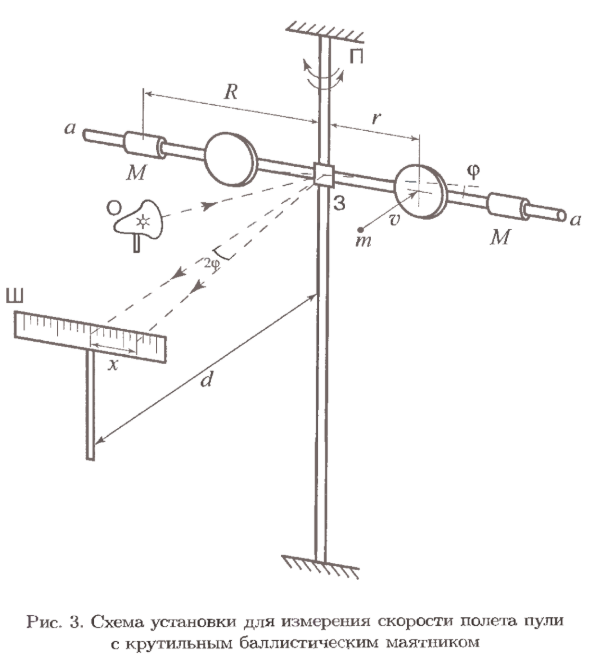
\includegraphics[scale=0.8]{1.2.1 3}
\end{center}



Законом созранения момента импульса можно воспользоваться, если время соударения пули с мишенью значительно меньше периода малых колебаний маятника. Поворот маятника при колебаниях. Соответственно мал момент кручения, возникающий при этом в проволоке, по сравнению с моментом при максимальном повороте, который всегда имеет конечную величину. Но главное -- мало произведение момента кручения в проволоке на время соударения по сравнению с моментом импульса, которым обладала пуля перед ударом.

Начальная кинетическая энергия вращения маятника переходит в потенциальную -- упругую энергию закручивания проволоки и расходуется на необратимые потери -- в первую очередь на трение о воздух. Роль потерь можно оценить по изменению амплитуды колебаний за 10 периолов. Если амплитуда уменьшается менее чем наполовину, то затухание колебаний считаем малым, то есть потери энергии за период колебаний значительно меньше энергии колебаний. Пренебрегая потерями, закон сохранения энергии при колебаниях записываем следующим образом: \[ k\frac{\varphi^2}{2} = I\frac{\Omega^2}{2}.\]

Здесь $k$ -- модуль кручения проволоки П, а $\varphi$ -- максимальный угол поворота маятника.\\
Из (6) и и(7) получаем \[ u = \varphi\frac{\sqrt{kI}}{mr}.\]

Угол максимального закручивания маятника в данных опытах всегда мал  и легко находится по смещения $x$ изоюражения нити осветителя на измерительной шкале. Из рис. 3 следует : \[ \varphi \approx \frac{x}{2d}.\]

Здесь $d$ -- расстояние от шкалы Ш до оси вращения маятника.\\
В формулу (8) входит произведение $kI$, которое можно найти по измерениям периодов колебаний маятника с грузами $M$ и без них. В первом случае период колебаний равен: \[ T_1 = 2\pi \sqrt{\frac{I}{k}}.\]

Во втором случае \[ T_2 = 2\pi \sqrt{\frac{I - 2MR^2}{k}}.\]

Из (10) и (11) следует \[ \sqrt{kI} = \frac{4\pi MR^2T_1}{T_1^2 - T_2^2}.\]

Здесь R -- расстояние от центров масс грузов $M$ до проволоки.

\begin{center}
{\bf Ход работы}
\end{center}
\begin{center}
{\bf 1. Знакомство с установкой}
\end{center}

Изучает и ознокамляемся с конструкцией установки,а так же научимся пользоваться духовым ружьем.
\begin{center}
{\bf 2. Измерение масс пуль}
\end{center}

Так как массы пуль для данной части уже измерены раньше, то просто предоставляю данные о пулях, с которыми будут проводиться дальнейшие измерения:  

\begin{center}
\begin{tabular}{|c|c|c|c|c|}
\hline 
m, гр & 0.509 & 0.510 & 0.500 & 0.505\\ 
\hline 
N & 1 & 2 & 3 & 4\\ 
\hline 
\end{tabular} 
\end{center}
\begin{center}
{\bf 3. Измерение данный об установке}
\end{center}

Измеряем с помощью линейки расстояния $r$, $R$, $d$(см. рис. 3).

\begin{center}
\begin{tabular}{|c|c|c|c|c|c|}
\hline 
r, см  & 20 & 20 & 20 & 20 & 20\\ 
\hline
R, см  & 33.8 & 33.8 & 33.8 & 33.8 & 33.8\\ 
\hline
d, см  & 56 & 56 & 56 & 56 & 56\\ 
\hline 
$N$  & 1 & 2 & 3 & 4 & 5\\ 
\hline
\end{tabular} 
\end{center}

Из таблицы, с учетом погрешности, получаем, что $r = 20 \pm 0.1$см, $R = 33.8 \pm 0.1$см, $d = 56 \pm 0.1$см.

Массы грузов, указанные на них: $M_1 = 725.6 $ гр , $M_1 = 736.8$ гр.
\begin{center}
{\bf 4. Настройка оптической системы}
\end{center}

Настраиваем оптическую система, предназначенную для измерения поворота маятника. Включаем осветитель О, направляем свет на зеркальце З и получаем четкое изображение нити осветителя на шкале.
\begin{center}
{\bf 5. Проверка реакции маятника на малое воздействие}
\end{center}

Производим несколько холостых выстрелов и убеждаемся, что маятник практически не реагирует на воздушную струю из ружья.
\begin{center}
{\bf 6. Малые затухания}
\end{center}

Так как период колебаний уменьшается на меньше чем 50$\%$, то мы убеждаемся в малом затухании колебаний.
\begin{center}
{\bf 7. Измерение периодов $T_1$ и $T_2$}
\end{center}

Измеряем время 10-15 полных крутильных колебаний маятника, при помощи секундомера, определяем $T_1$ и $T_2$. По формуле (12) находим величину $\sqrt{kI}$ и оценим ее погрешность. Измеряем периоды несколько раз, чтобы получить более точные данные. Таблица полученных данных $T$ :

\begin{center}
\begin{tabular}{|c|c|c|c|c|}
\hline 
$10T_1$, c& 155 & 155 & 155 & 155 \\ 
\hline 
$10T_2$, c& 125 & 125 & 125 & 125 \\ 
\hline 
$T_1$, c& 15.5 & 15.5 & 15.5 & 15.5 \\ 
\hline 
$T_2$, c& 12.5 & 12.5 & 12.5 & 12.5 \\ 
\hline 
$N$ & 1 & 2 & 3 & 4 \\ 
\hline 
\end{tabular} 
\end{center}

Так как периоды $T$ измерялись с помощью телефонного секундомера, то $\sigma_T = 0.01$ c. Все 4 раза измерения $T_1$ и $T_2$ дали практически одинаковый результат, поэтому их случайной погрешностью можно пренебречь. $2M = M_1+M_2 \Rightarrow M = 0.731$ кг. Тогда $\sqrt{kI} = \frac{4\pi MR^2 T_1}{T_1^2 - T_2^2} = 0.194$        . Погрешность $\sigma_M = 0.005$ кг, $\sigma_R = 0.001$ м . Так как $\sqrt{kI}$ в основном зависит от $M$ и $R$, а $T_1$ и $T_2$ практически константы, то :  

\[\sigma_{\sqrt{kI}} = \sqrt{(\frac{\sigma t}{\sigma M})^2\cdot \sigma_M^2 + (\frac{\sigma t}{\sigma R})^2\cdot \sigma_R^2}.\]

Тогда погрешность :

\[\sigma_{\sqrt{kI}} = \sqrt{\frac{4\pi R^2 T_1}{T_1^2 - T_2^2} \cdot \sigma_M^2 + \frac{2\cdot 4\pi MRT_1}{T_1^2 - T_2^2}\cdot \sigma_R^2} = \sqrt{(6.62+ 1.15)\cdot 10^{-6}} = 2.8\cdot 10^{-3}.\]


\begin{center}
{\bf 8. Измерение скорости пули}
\end{center}

Проводим несколько выстрелов, замеряем $x$, зная $\sqrt{kI}$ и по формулам определяем скорость пули при каждом выстреле. Таблица полученных данных: 
\begin{center}
\begin{tabular}{|c|c|c|c|c|}
\hline 
$N$ & 1 & 2 & 3 & 4 \\ 
\hline 
$m$, гр & 0.509 & 0.510 & 0.5 & 0.505 \\ 
\hline 
$x$, см & 10 & 10.5 & 9.5 & 10 \\ 
\hline 
\end{tabular} 
\end{center}

Отсюда получаем таблицу данных для $u$ :

\begin{center}
\begin{tabular}{|c|c|c|c|c|}
\hline 
$N$ & 1 & 2 & 3 & 4 \\ 
\hline 
$u$, м/с & 170 & 178.3 & 164.6 & 171.5 \\ 
\hline  
\end{tabular} 
\end{center}


\begin{center}
{\bf 9. Оценка погрешностей}
\end{center}

Оцениваем погрешность определения скорости пули в каждом выстреле по полученным данным.

\[u = \varphi \frac{\sqrt{kI}}{mr},\ \sigma_u = \sqrt{(\frac{\sqrt{kI}}{mr})^2\cdot \sigma_{\varphi}^2 + (\frac{\varphi}{mr})^2\cdot \sigma_{\sqrt{kI}}^2 + (\frac{\varphi \sqrt{kI}}{m^2r})^2\cdot \sigma_{m}^2    + (\frac{\varphi \sqrt{kI}}{mr^2})^2\cdot \sigma_{r}^2 }.\]

\[ \sigma_{\varphi} = \sqrt{ (\frac{1}{2d})^2\cdot \sigma_x^2 +(\frac{x}{2d^2})^2\cdot \sigma_d^2 }  .\]
 
По вышеприведенным формулам получаем, что $\sigma_{\varphi} = 0.85 \cdot 10^{-3}$ ,тогда $ \sigma_u \approx 3.4$ м/с.
\newpage
\begin{center}
{\bf 10. Оценка разброса и среднего значения скорости пули}
\end{center}

Находим среднее значение скорости пули и разброса отдельных результатов около среднего значения.

$\langle u\rangle = 171.1$ м/с.

$\Delta_1 = |171.1 - 170| = 1.1$ м/с.

$\Delta_2 = |171.1 - 178.3| = 7.2$ м/с.

$\Delta_3 = |171.1 - 164.6| = 6.5$ м/с.

$\Delta_4 = |171.1 - 171.5| = 0.4$ м/с.

{\bf Вывод}

Полученные значения скорости пули в разных частях не совсем совпадают в границах погрешности. Полученный разброс связан в основном с разной скоростью от выстрела к выстрелу ружья(так как разные части лабораторной работы производились при помощь разных ружьев, а скорость выстрела на прямую зависит от накаченности баллона).Так же она сильно варьируется из-за разных форм пуль и других различных факторов . Так же можно сказать, что результат частично связан с погрешностью измерений и используемых приближений при проведении работы.

Поэтому нельзя делать выводы об скорости пули, потому что она очень сильно зависит от накаченности баллона в нашем ружье. Средни скорости пуль для определенного ружья  можно определить как :

\[u = \langle u\rangle \pm\ \sigma_u\].

\end{document}


